\chapter{Validation} \label{chap:validation}

\section*{}

% To validate the framework 3 testbeds were prepared. The first is a collection 
% of small fabricated test cases where we compare the output of multiple 
% simulation runs to the expected results. The second and third cases deal with 
% real uses of the framework, applied in two different e-commerce contexts: the 
% first is an online store of computer products and the second is a general 
% comparison shopping website.

To validate the framework 2 testbeds were prepared. The first is a collection 
of small fabricated test cases where we compare the output of multiple 
simulation runs to the expected results. The second case deals with a real use 
of the framework, applied to an online store.

% \section{Validation methodology}

\section{Sanity checks} % rename?

\subsection{Expected number of agents in the simulation}

This test compares the number of navigation agents expected to be 
\textit{alive} at each simulation step with the actual number of them.

At each simulation step, $k$ navigation agents enter the system and  
$p_{exit}$ of them leaves, which leads to the recurrence equation \ref{eq:recc}.

\begin{equation}\label{eq:recc}
\begin{cases}
a_{1} = \left (1 - p_{exit}  \right ) k\\
a_{n} = \left (1 - p_{exit}  \right ) \left (k + a_{n - 1} \right)
\end{cases} \Leftrightarrow a_{n} = \frac{k (p_{exit}-1) ((1-p_{exit})^{n} - 
1)}{p_{exit}}
\end{equation}

The simulation run was configured in the following way:

\begin{itemize}
    \item \textbf{Website}: Sample website with 9 pages and 32 total links 
    between pages
    \item \textbf{Website agent}: Dummy agent, does not modify any page;
    \item \textbf{Navigation agent}: Sample agent implementation with a chance 
    of exiting the website of $\frac{1}{3}$ ($p_{exit}$);
    \item \textbf{Number of new navigation agents each step}: 100 ($k$)
    \item \textbf{Number of simulation steps}: 1000
\end{itemize}

Replacing the values in equation \ref{eq:recc}: $a_{n} = -200 \left ( 
\frac{2}{3}^{n} - 1 \right )$. After a few simulation runs, the expected number 
of agents in the system stabilizes: $\lim_{n\to \infty} -200 \left ( 
\frac{2}{3}^{n} - 1 \right ) = 200$.

The results of a simulation run were gathered and plotted in figure 
\ref{fig:expagents}. Triangles ($\triangle$) represent the actual value 
($A_{t}$) and circles ($\bullet$) represent the expected value ($E_{t}$) 
according to the equations above. SMAPE (symmetric mean absolute percentage 
error)\cite{makridakis1993accuracy} is used to measure the accuracy of the 
results: $ SMAPE = {\frac {1}{n}}\sum _{t=1}^{n}{\frac 
{\left|E_{t}-A_{t}\right|}{|A_{t}|+|E_{t}|}} = 3.07\% $, which is a reasonable 
low \textit{error} rate given the randomness of the system.

\begin{figure}[h]
    \begin{center}
        \leavevmode
        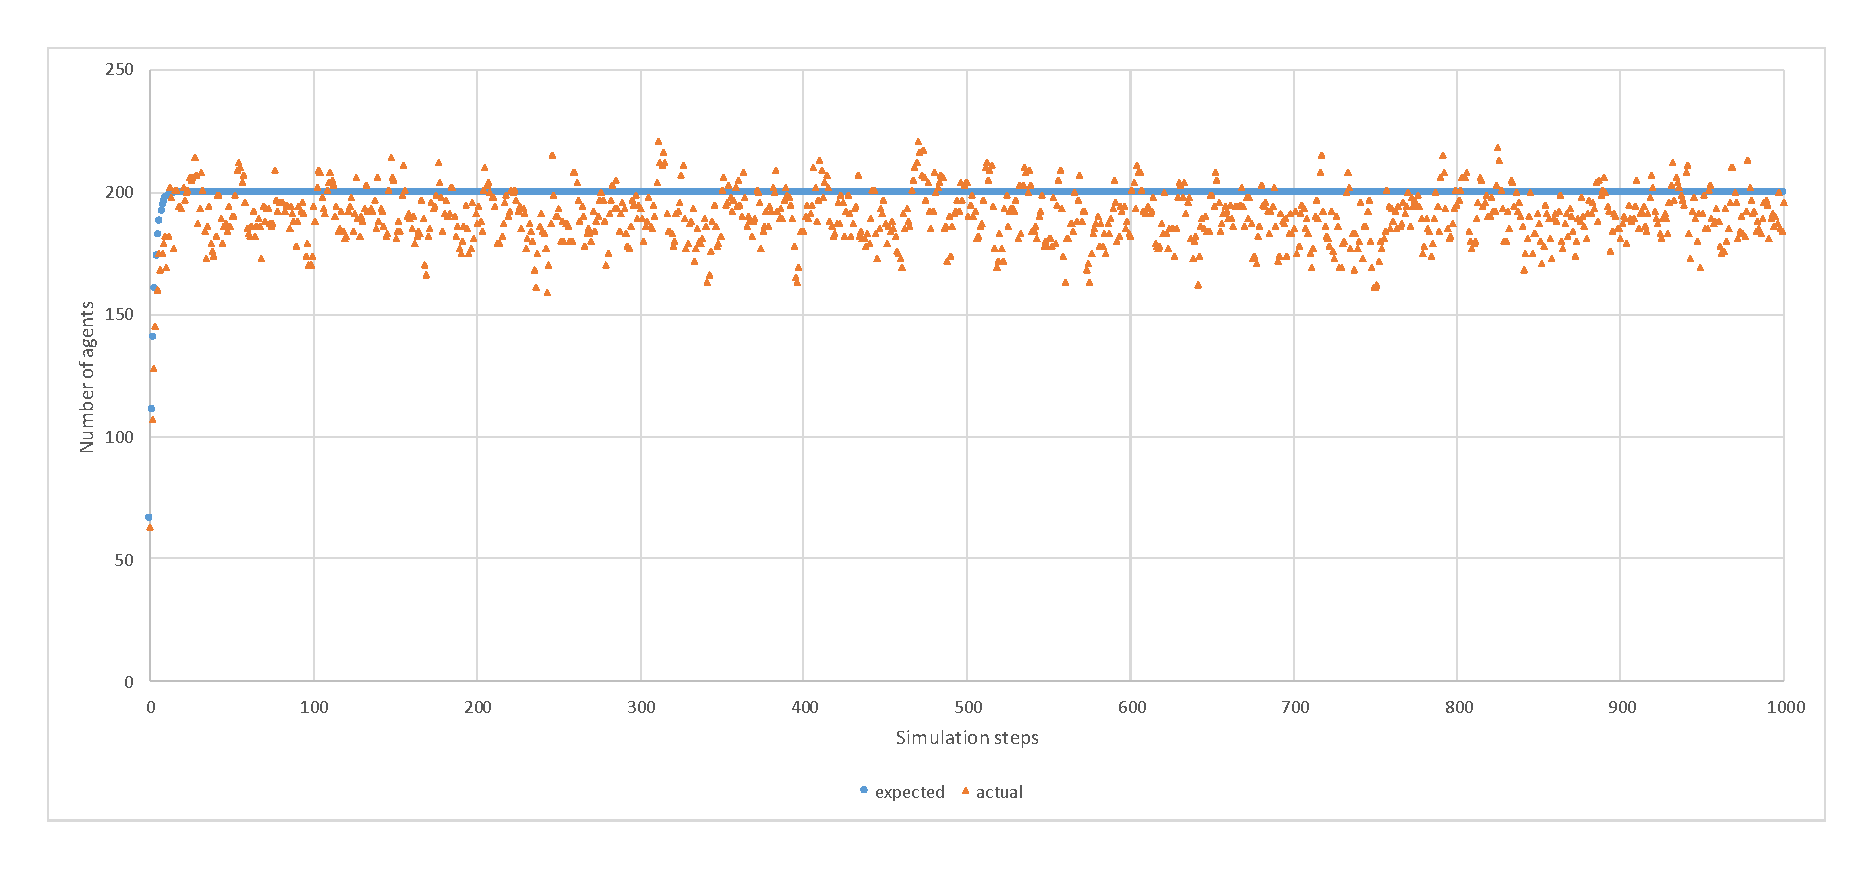
\includegraphics[width=1\textwidth]{expected_agents}
        \caption{Expected number of agents in the simulation}
        \label{fig:expagents}
    \end{center}
\end{figure}

\subsection{Expected number of visits}

This test compares the number of visits (page hits) for a given website and 
agents setup. The simulation run was configured in the following way:

\begin{itemize}
    \item \textbf{Website}: Website configured as displayed in figure 
    \ref{fig:test2website}. The homepage links to 5 product pages and the 
    product page link to the cart page.
    \item \textbf{Website agent}: Dummy agent, does not modify any page;
    \item \textbf{Navigation agent}: The agent picks one linked page randomly, 
    however, if current page is for a product, it always buys it. If the 
    current page is the cart page, it leaves the website;
    % \todo{algorithm?}
    \item \textbf{Number of new navigation agents each step}: 100
    \item \textbf{Number of simulation steps}: 1000
\end{itemize}

\begin{figure}
    \centering
    \begin{tikzpicture}
        \SetGraphUnit{3}
        \GraphInit[vstyle=Welsh]
        \tikzset{VertexStyle/.append style = { minimum size = 24pt}}
        \Vertex{page3}
        \WE(page3){page2}
        \WE(page2){page1}
        \EA(page3){page4}
        \EA(page4){page5}
        \NO(page3){homepage}
        \SO(page3){cart}
        \tikzset{EdgeStyle/.append style = {->}}
        \Edge(homepage)(page1)
        \Edge(homepage)(page2)
        \Edge(homepage)(page3)
        \Edge(homepage)(page4)
        \Edge(homepage)(page5)
        \tikzset{EdgeStyle/.append style = {->}}
        \Edge(page1)(cart)
        \Edge(page2)(cart)
        \Edge(page3)(cart)
        \Edge(page4)(cart)
        \Edge(page5)(cart)
        % \tikzset{EdgeStyle/.append style = {->,bend left}}
        % \Edge(cart)(homepage)
    \end{tikzpicture}
    \caption{Website graph for the expected visits test} 
    \label{fig:test2website}
\end{figure}

The table \ref{tab:test2results} displays the expected and observed number of 
visits for a simulation run as described above. The percent error is calculated 
and the obtained results are very close to the predicted values.

\begin{table}[]
    \centering
    \caption{Expected and observed number of visits}
    \label{tab:test2results}
    \begin{tabular}{@{}lllll@{}}
        \toprule
        Page     & Observed   & \multicolumn{2}{l}{Expected} & Error  \\ 
        \midrule
        homepage & $100000$   & $100 \times 1000$ & $ = 100000$      & $0.00\%$ 
        \\
        page1    & $19864$    & $\frac{1}{5} \times 100 \times 1000$ & $ = 
        20000$ &         $0.68\%$ \\
        page2    & $20100$    & $\frac{1}{5} \times 100 \times 1000$ & $ = 
        20000$ &         $0.50\%$ \\
        page3    & $19696$    & $\frac{1}{5} \times 100 \times 1000$ & $ = 
        20000$ &         $1.52\%$ \\
        page4    & $20096$    & $\frac{1}{5} \times 100 \times 1000$ & $ = 
        20000$ &         $0.48\%$ \\
        page5    & $20244$    & $\frac{1}{5} \times 100 \times 1000$ & $ = 
        20000$ &         $1.22\%$ \\
        cart     & $99900$    & $20000 \times 5$ & $ = 100000$       & $0.10\%$ 
        \\ 
        \bottomrule
    \end{tabular}
\end{table}

\subsection{Expected bounce rate}

This case compares the bounce rate for a website that only has one page. We 
define the bounce rate as the percentage of navigation agent sessions that only 
view a single page before existing the website.

The simulation run was configured in the following way:

\begin{itemize}
    \item \textbf{Website}: One page only, the homepage;
    \item \textbf{Website agent}: Dummy agent, does not modify any page;
    \item \textbf{Navigation agent}: Agent that picks its actions randomly;
    \item \textbf{Number of new navigation agents each step}: 100
    \item \textbf{Number of simulation steps}: 1000
\end{itemize}

As expected, the simulation results yield $100\%$ bounce rate, all of the 
visits were to the homepage, $10000$ unique users ($100 \times 1000$) and no 
purchases, as it can be seen on figure \ref{fig:test3result}.

\begin{figure}[h]
    \begin{center}
        \leavevmode
        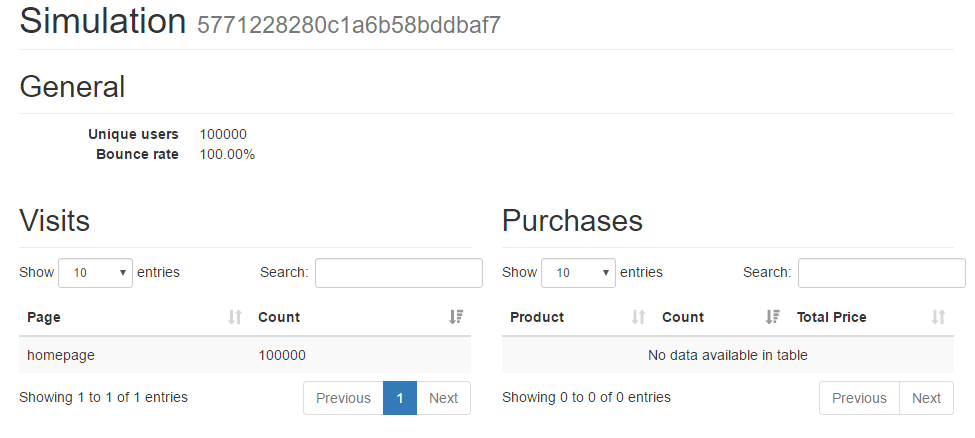
\includegraphics[width=1\textwidth]{expected_bounce_rate}
        \caption{Screenshot of the frontend results for this test run}
        \label{fig:test3result}
    \end{center}
\end{figure}

% \subsection{ test conversion rate, always buy -> 100% }

\section{Online store}

This test case uses data from a real online store that sells electronics and 
computers products. This website presents a fairly standard online store, 
mostly consisting of product listing and product pages. There are 3 places 
where it is possible to recommend products: the homepage has two sections, one 
with product highlights and another with product promotions and each product 
page has a tab to show related products.

\subsection{Input data and configuration}

The website consists of 2540 pages with 343201 links between pages, spanning 25 
base product categories and 103 sub-categories. There are 750 product list 
pages, 1748 product pages, 1 cart page and 41 uncategorised/generic pages, 
visualised in figure \ref{fig:cfcategories}.

\begin{figure}[h]
    \begin{center}
        \leavevmode
        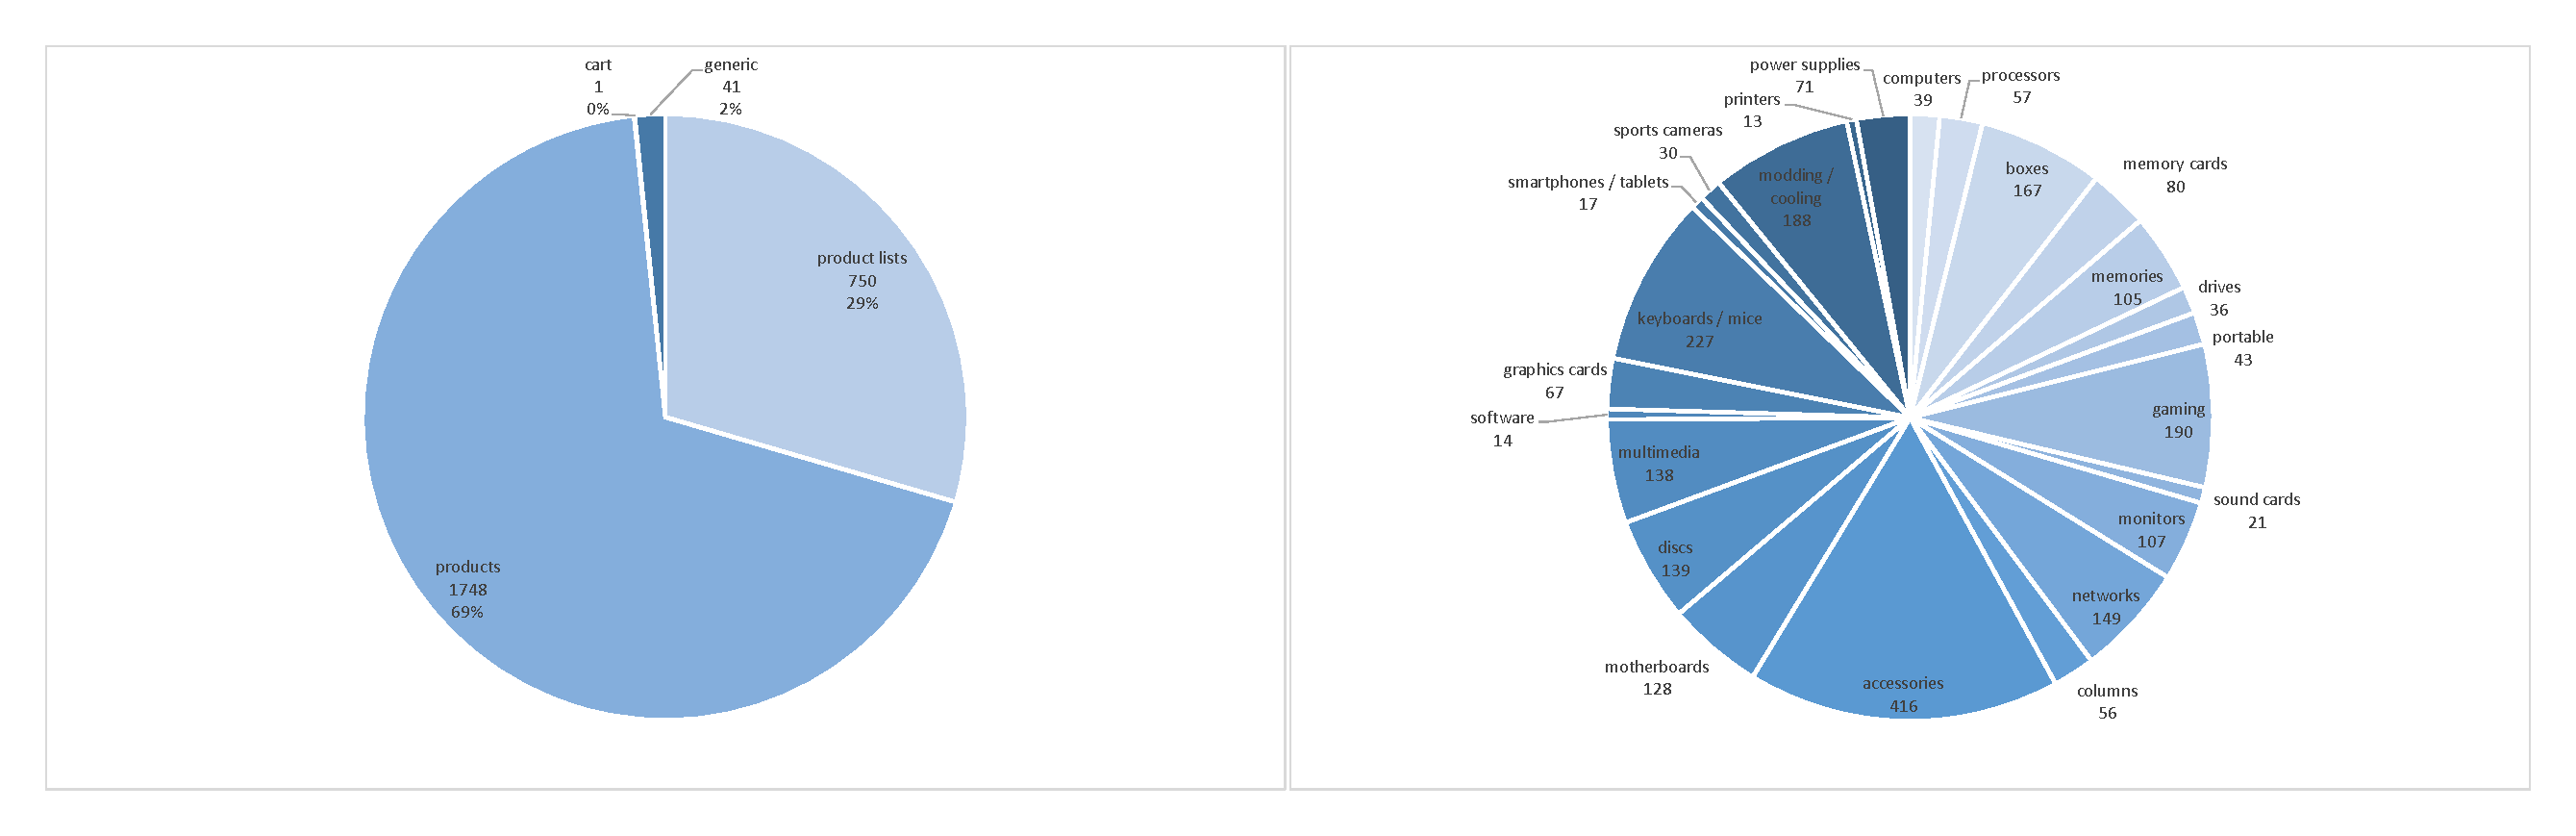
\includegraphics[width=1\textwidth]{cf_categories}
        \caption{Distribution of the type of pages in the website (left) and 
        distribution of the categories of the products (right)}
        \label{fig:cfcategories}
    \end{center}
\end{figure}

To simulate users and customers (the \texttt{NavigationAgent}s) interacting 
with this particular website, a model based on affinities was built. This model 
is composed by the \textit{affinities} themselves (a mapping between product 
categories and the likelihood of the user liking or having interest on products 
of that category), the probability of buying a product, the probability of 
exiting the website and the arrival rate.

Because real usage website data is not available for this website, a sample 
profile was created with the following properties: the affinities were set up 
as displayed in table \ref{tab:sample_user}, probability of buying set to 
$5\%$, probability of leaving the website of $15\%$ and a rate of arrival to 
the website following a \textit{Poisson} distribution with $\lambda = 500$.

\begin{table}[h]
    \centering
    \caption{Affinities for a sample user}
    \label{tab:sample_user}
    \begin{tabular}{@{}ll@{}}
        \toprule
        \textbf{Category}  & \textbf{Weight}  \\ \midrule
        Computadores       & 14.29\% \\
        MSI                & 14.29\% \\
        Pen Drives         & 7.14\%  \\
        Portáteis          & 14.29\% \\
        Intel 2011         & 14.29\% \\
        Cartões de Memória & 7.14\%  \\
        Brand              & 14.29\% \\
        Processadores      & 14.29\% \\ \bottomrule
    \end{tabular}
\end{table}

\subsection{Simulation}

The simulation was configured as described in the subsection above. All the 
navigation agents use the same profile. The "thought" process for each agent is 
fairly simple: at each step, they try to buy a product and exit the website in 
accordance to the probabilities defined \textit{a priori} or navigate to a 
different page based on their categories, with preference as stated by the 
affinity table. The simulation was run for 30 steps.

\subsection{Results}

The results of a sample simulation run are summarized in the tables 
\ref{tab:visitscat} and \ref{tab:genstats}. They are expected: the number of 
unique users is 14894 and the expected value is 15000 ($500 \times 25$); the 
bounce rate is $14.58\%$ and the prior leaving rate is $15\%$; and the 
conversion rate is $4.77\%$ and the prior buy rate is $5\%$.

\begin{table}[h]
    \centering
    \caption{Visits per category for a sample simulation run}
    \label{tab:visitscat}
    \begin{tabular}{@{}lll@{}}
        \toprule
        \textbf{Category}                   & \textbf{Sub-category} & 
        \textbf{Count} \\ \midrule
        \multirow{5}{*}{Cartões de Memória} & Pen Drives            & 
        6492           \\
        & SD/MiniSD/MicroSD     & 1203           \\
        & Leitor de Cartões     & 1199           \\
        & Compact Flash         & 1158           \\
        & -                     & 37             \\ \midrule
        \multirow{4}{*}{Portáteis}          & MSI                   & 
        14326          \\
        & HP                    & 2623           \\
        & Asus                  & 2584           \\
        & -                     & 263            \\ \midrule
        \multirow{5}{*}{Processadores}      & Intel 2011            & 
        7097           \\
        & Intel 1151            & 2752           \\
        & Intel 1150            & 2379           \\
        & AMD                   & 2234           \\
        & -                     & 240            \\ \midrule
        \multirow{2}{*}{Computadores}       & Brand                 & 
        19802          \\
        & -                     & 188            \\ \midrule
        Motherboards                        & Intel 2011            & 
        4917           \\ \bottomrule
    \end{tabular}
\end{table}

\begin{table}[h]
    \centering
    \caption{Metrics/info regarding a sample simulation run}
    \label{tab:genstats}
    \begin{tabular}{@{}ll@{}}
        \toprule
        \textbf{Field}  & \textbf{Value}               \\ \midrule
        Unique users    & 14894                        \\
        Bounce rate     & 14.58\%                      \\
        Conversion rate & 4.77\%                       \\
        Purchases       & 676                          \\
        NavAgentFactory & AffinityFactory              \\
        NavAgent        & AffinityUser                 \\
        WebsiteAgent    & DummyWebsiteAgent            \\
        Start time      & Thu Jul 07 14:14:36 BST 2016 \\
        End time        & Thu Jul 07 14:14:39 BST 2016 \\ \bottomrule
    \end{tabular}
\end{table}

%\section{Comparison shopping website}

%\todo{...}

%\subsection{Input data and configuration}
%\subsection{Simulation}
%\subsection{Results}
